% !TeX root = main.tex
\section{Methodology} \label{sec:method}

\subsection{Setting and Participants}
The research was conducted within an Artificial Intelligence (AI) elective course, consisting of three credits, during the Fall semester of 2023 at a large private university in India. The study involved 105 sophomore and junior undergraduate students pursuing computer science and information systems degrees. Among the participants, 98 were male, and 7 were female, all within the age range of 18 to 21 and hailing from India. The course employed a continuous evaluation method, with 30\% allocated to assignments, quizzes, and research reading, 30\% to a mid-term closed-book examination, and 40\% to a comprehensive final examination at the end of the term.

\subsection{Measures}
The following measures were used in the study:
\subsubsection{The International Personality Item Pool (IPIP)}
The International Personality Item Pool (IPIP)\footnote{\url{https://ipip.ori.org/}} stands as a comprehensive resource for personality assessment items, facilitating research in psychology across diverse cultural settings. Established in the 1990s by Goldberg \cite{Goldberg}, the IPIP offers an extensive array of self-report measures to assess various dimensions of personality, including the Big Five traits: openness, conscientiousness, extraversion, agreeableness, and neuroticism. In this study, participants Big Five personality traits were evaluated using the rigorous and comprehensive 120-item version of the IPIP \cite{JOHNSON201478}. This choice was made because the 120-item version strikes a balance, being neither too brief (like the 50-item version) nor overly extensive (like the 300-item version), thus enabling completion within a reasonable timeframe of less than 30 minutes, which is suitable for students.

The 120-item version of the IPIP scale comprises 24 items for each subscale, totaling 120 items. Participants assess the degree to which each item (question or statement) reflects their personality on a 5-point Likert scale, ranging from 1 = very inaccurate to 5 = very accurate. The internal consistency coefficients (Cronbach's alpha) for the five subscales ranged from \begin{math} \alpha \end{math} = 0.84 to 0.93, with values for extraversion at 0.92, agreeableness at 0.85, conscientiousness at 0.84, neuroticism at 0.90, and openness to experience at 0.93. These coefficients signify the reliability of the scale in measuring each personality trait, with higher values indicating greater internal consistency among the items within each subscale.

\subsubsection{Plagiarism Detection}
The Measure of Software Similarity (MOSS) tool \cite{MOSS} was used to detect plagiarism in the programming assignments. MOSS provided a percentage-based measure of similarity between code submissions, allowing for the calculation of plagiarism scores for each assignment. 

\subsection{Research Design}
As depicted in Figure \ref{fig:activityTimeline}, at the onset of the semester, participants voluntarily underwent a Big Five personality trait assessment test, with their scores for each trait recorded for subsequent analysis. X weeks into the semester, participants were given the first programming assignment without any explicit guidance or instructions regarding plagiarism (apart from action to malpractice action shared in the course handout and in the institute policy). The data on personality traits and plagiarism scores, obtained through the Measure of Software Similarity (MOSS) for assignment 1, were utilized to address research question RQ\ref{RQ1}.

\begin{figure}[ht]
  \centering
  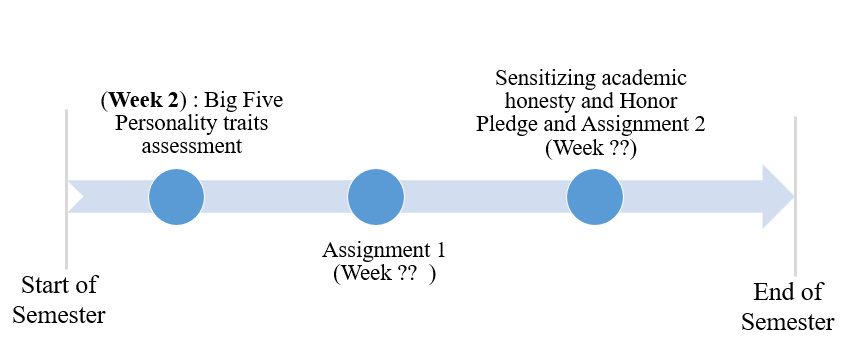
\includegraphics[width=\columnwidth]{2.png}
  \caption{Series of activities}
  \label{fig:activityTimeline}
\end{figure}

The second programming assignment was issued X weeks subsequent to the completion of the initial assignment. Participants were requested to read and endorse an integrity pledge concerning plagiarism, alongside the assignment instructions. This was aimed at raising awareness about the concept of plagiarism and upholding academic integrity. It explicitly outlined the behaviors considered plagiarism. The pledge was administered via a google form and mandated a digital signature from each participant, signifying their commitment to refrain from plagiarism in the upcoming assignment. We adopted this approach to raise students' awareness of what constitutes plagiarism, rather than conducting a classroom session. Our institute's zero percentage attendance policy influenced this decision, ensuring that this crucial information reaches all students. An excerpt from the integrity pledge is presented below:

\begin{myquote}
    \textit{The assignments are to be done individually by each student. The objective of the assignments is to help students deepen their understanding of some of the concepts. A secondary objective of the assignments is to help students get better at Python programming.}
    \textbf{Each} of the following amounts to violations of academic integrity:
    \begin{itemize}
        \item \textit{Sharing a part or whole of your program with another student even if one of the students changes the variable names and function names and rearranges the functions within the program file.}
        \item \textit{Sharing a part or whole of your report with another student even if one of the students changes most of the sentences so that superficially, the reports look different. You must cite the resources you have referred in the report.} 
        \item \textit{Getting parts of your program from past programming assignment submissions or internet sources. Each student must do the assignment individually.}
        \item \textit{Sharing code for commonly needed functionality by calling it "driver program" amounts to a violation of academic integrity because one of the objectives of this assignment is to help students get better at Python programming. }
    \end{itemize}
\end{myquote}
This assignment served as the post-intervention assessment, allowing for evaluating the impact of plagiarism awareness on participant behavior.

\subsection{Procedures for data collection and analysis}
\subsubsection{Personality Traits Data:} Following the institute's ethics policy, participants were required to provide informed consent before participating in the study. Upon obtaining consent, participants underwent the International Personality Item Pool (IPIP) personality test, which assesses the Big Five personality traits. The test was administered through an online tool available at the provided URL\footnote{\url{https://bigfive-test.com/}}.

After completing the test, participants' final scores for each Big Five personality trait were recorded in a Google form. To ensure confidentiality and protect participants' privacy, all data collected was anonymized, meaning any personally identifiable information was removed or obscured. Subsequently, the anonymized data was securely stored in a cloud-based platform for further analysis and processing.

\subsubsection{Assignment Data:} 
Both assignments were administered using Moodle, the institute's learning management system. Upon completion, the source codes for both assignments were subjected to analysis using the Measure of Software Similarity (MOSS) tool to generate plagiarism reports.

To ensure confidentiality, the data was anonymized before processing. The plagiarism scores corresponding to each student, derived from the MOSS reports, were then stored in cloud storage for subsequent analysis.The plagiarism score for each student was calculated based on the proportion of code similarity detected by MOSS. Specifically, it was determined by dividing the maximum number of lines copied from other sources by the total number of lines in the student's source code. This approach provided a quantitative measure of the extent of plagiarism in each student's assignment






